\documentclass[11pt,a4paper]{article}
\usepackage[margin=0.9in]{geometry}
\usepackage[T1]{fontenc}
\usepackage[utf8]{inputenc}
\usepackage{graphicx}
\usepackage{hyperref}
\usepackage{enumitem}
\usepackage{float}
\usepackage{amsmath}

\title{Advanced Image Processing Methods\\Homework 5 Report}
\author{Peter Dobosi}
\date{\today}

\begin{document}
\maketitle

\section*{Goal}
Build a complete PyTorch transfer-learning image-classification pipeline: load a \texttt{torchvision} dataset, fine-tune a pretrained model, validate with early stopping, then evaluate the best checkpoint on a held-out test set.

\section*{Method}
\begin{enumerate}[leftmargin=*,itemsep=1pt,topsep=2pt]
    \item \textbf{Data preparation}: The Describable Textures Dataset (DTD) is loaded through \texttt{torchvision}, using official \texttt{partition=1}: 1880 train, 1880 validation, and 1880 test images across 47 texture classes.
    Training images are resized to $224\times224$ and augmented online with random horizontal flip, rotation, and colour jitter; validation and test images use only resize, tensor conversion, and ImageNet normalisation.

    \item \textbf{Model}: The backbone is MaxViT-T with ImageNet pretrained weights. The final classifier layer is replaced by a 47-way \texttt{Linear} layer, and all 30.43M parameters remain trainable for full fine-tuning.

    \item \textbf{Training}: The model is trained with \texttt{CrossEntropyLoss} and Adam. After every epoch, validation is run under \texttt{model.eval()} and \texttt{torch.no\_grad()}. Early stopping monitors validation loss and saves only the best checkpoint.

    \item \textbf{Evaluation}: The best checkpoint is reloaded before test evaluation. The script reports test loss and accuracy, saves train/validation curves, and plots a 47-class confusion matrix for test predictions.
\end{enumerate}

The main hyperparameters were: image size $224\times224$, CUDA batch size 32, Adam learning rate $10^{-4}$, weight decay $10^{-4}$, 30 epoch budget, and early-stopping patience 5. The final run used Kaggle's Tesla T4 environment with PyTorch 2.10.0+cu128.

\section*{Results}
Training stopped after epoch 14. The best validation checkpoint was reached at epoch 9 with validation loss 1.0349 and validation accuracy 0.7234. On the test split, the reloaded best model achieved \textbf{72.71\% accuracy} with test loss \textbf{1.0189}. The curves show rapid transfer-learning convergence followed by mild overfitting: training loss keeps decreasing after epoch 9, while validation loss plateaus and then rises slightly.

\clearpage

\begin{figure}[H]
    \centering
    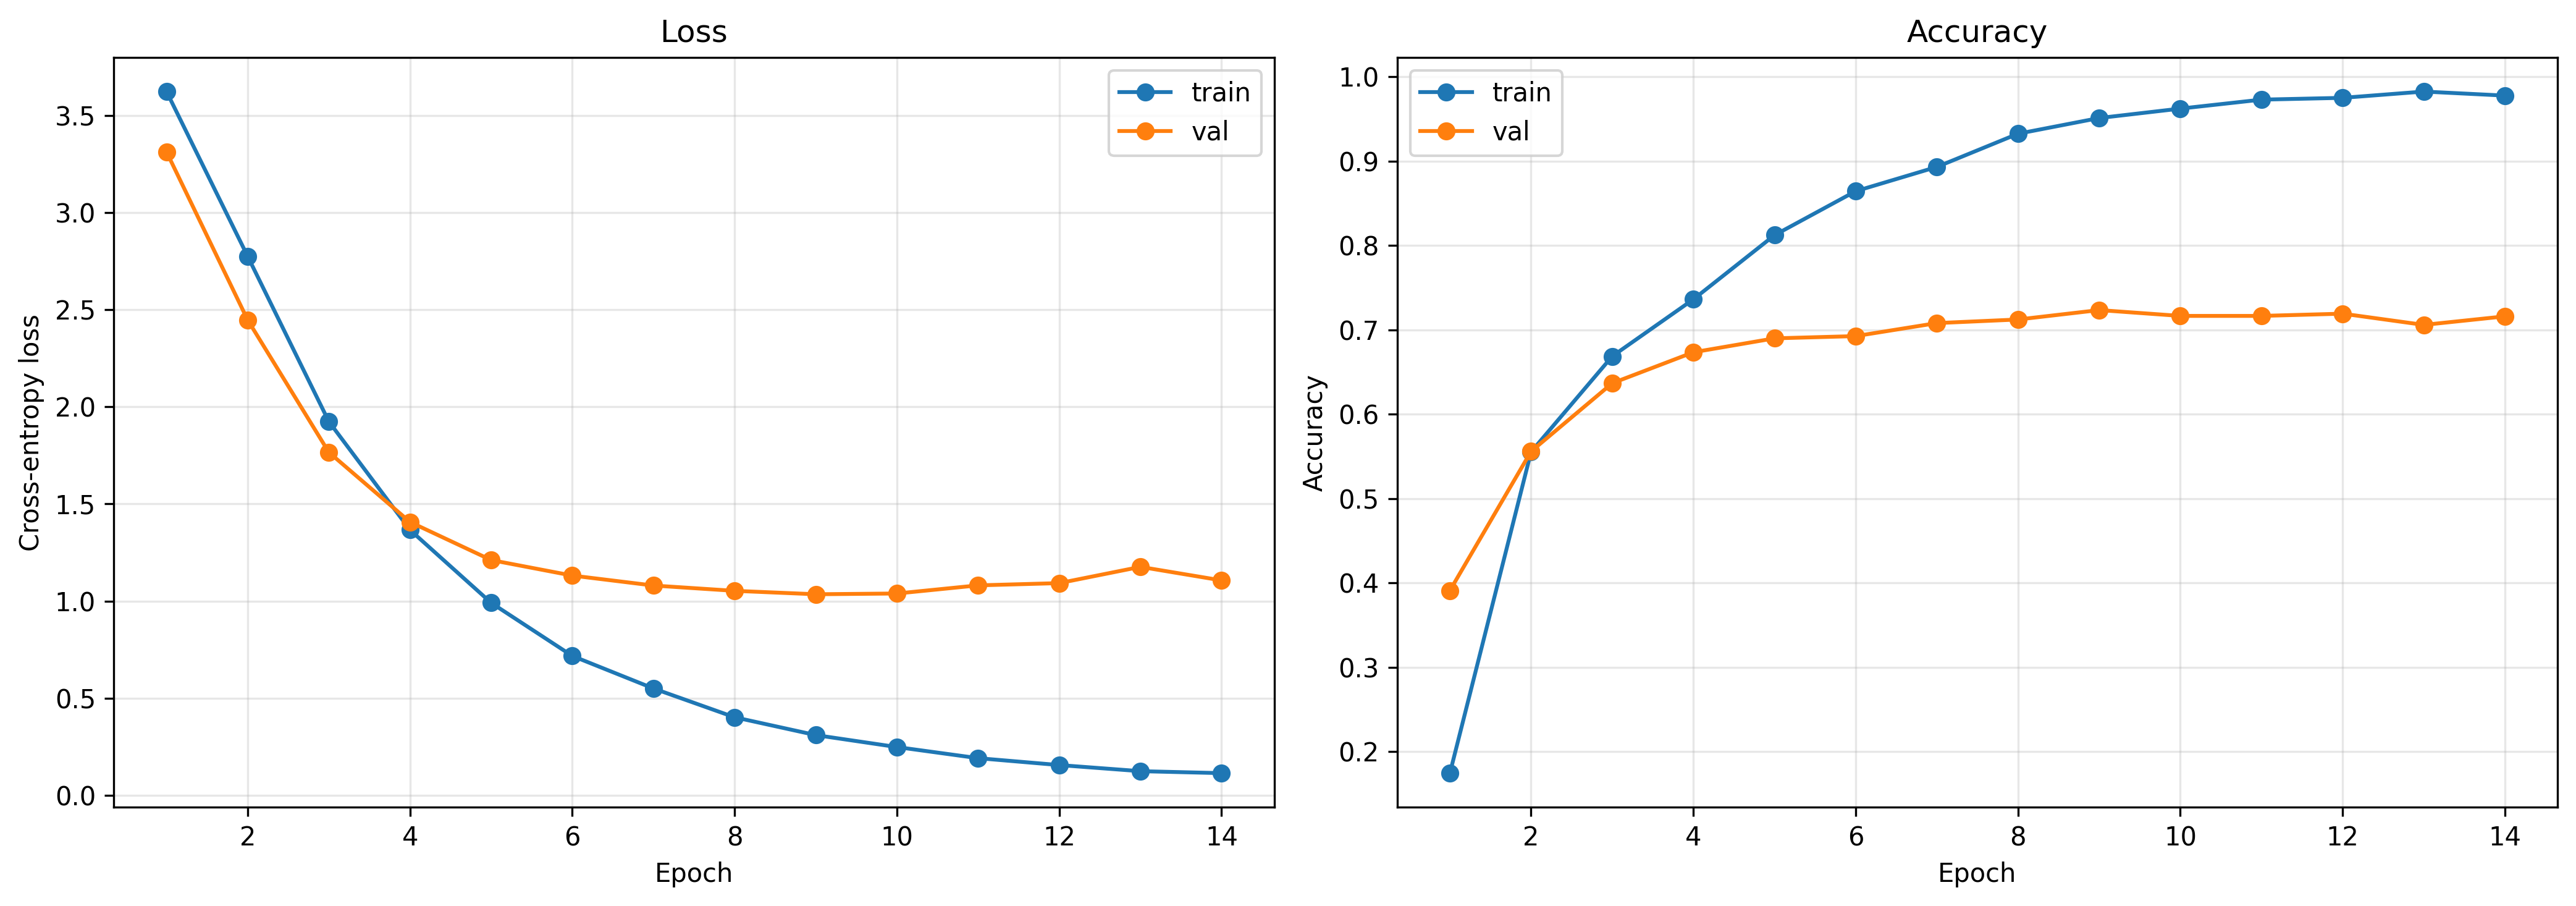
\includegraphics[height=2.0in]{output/training_curves.png}

    \vspace{0.2em}
    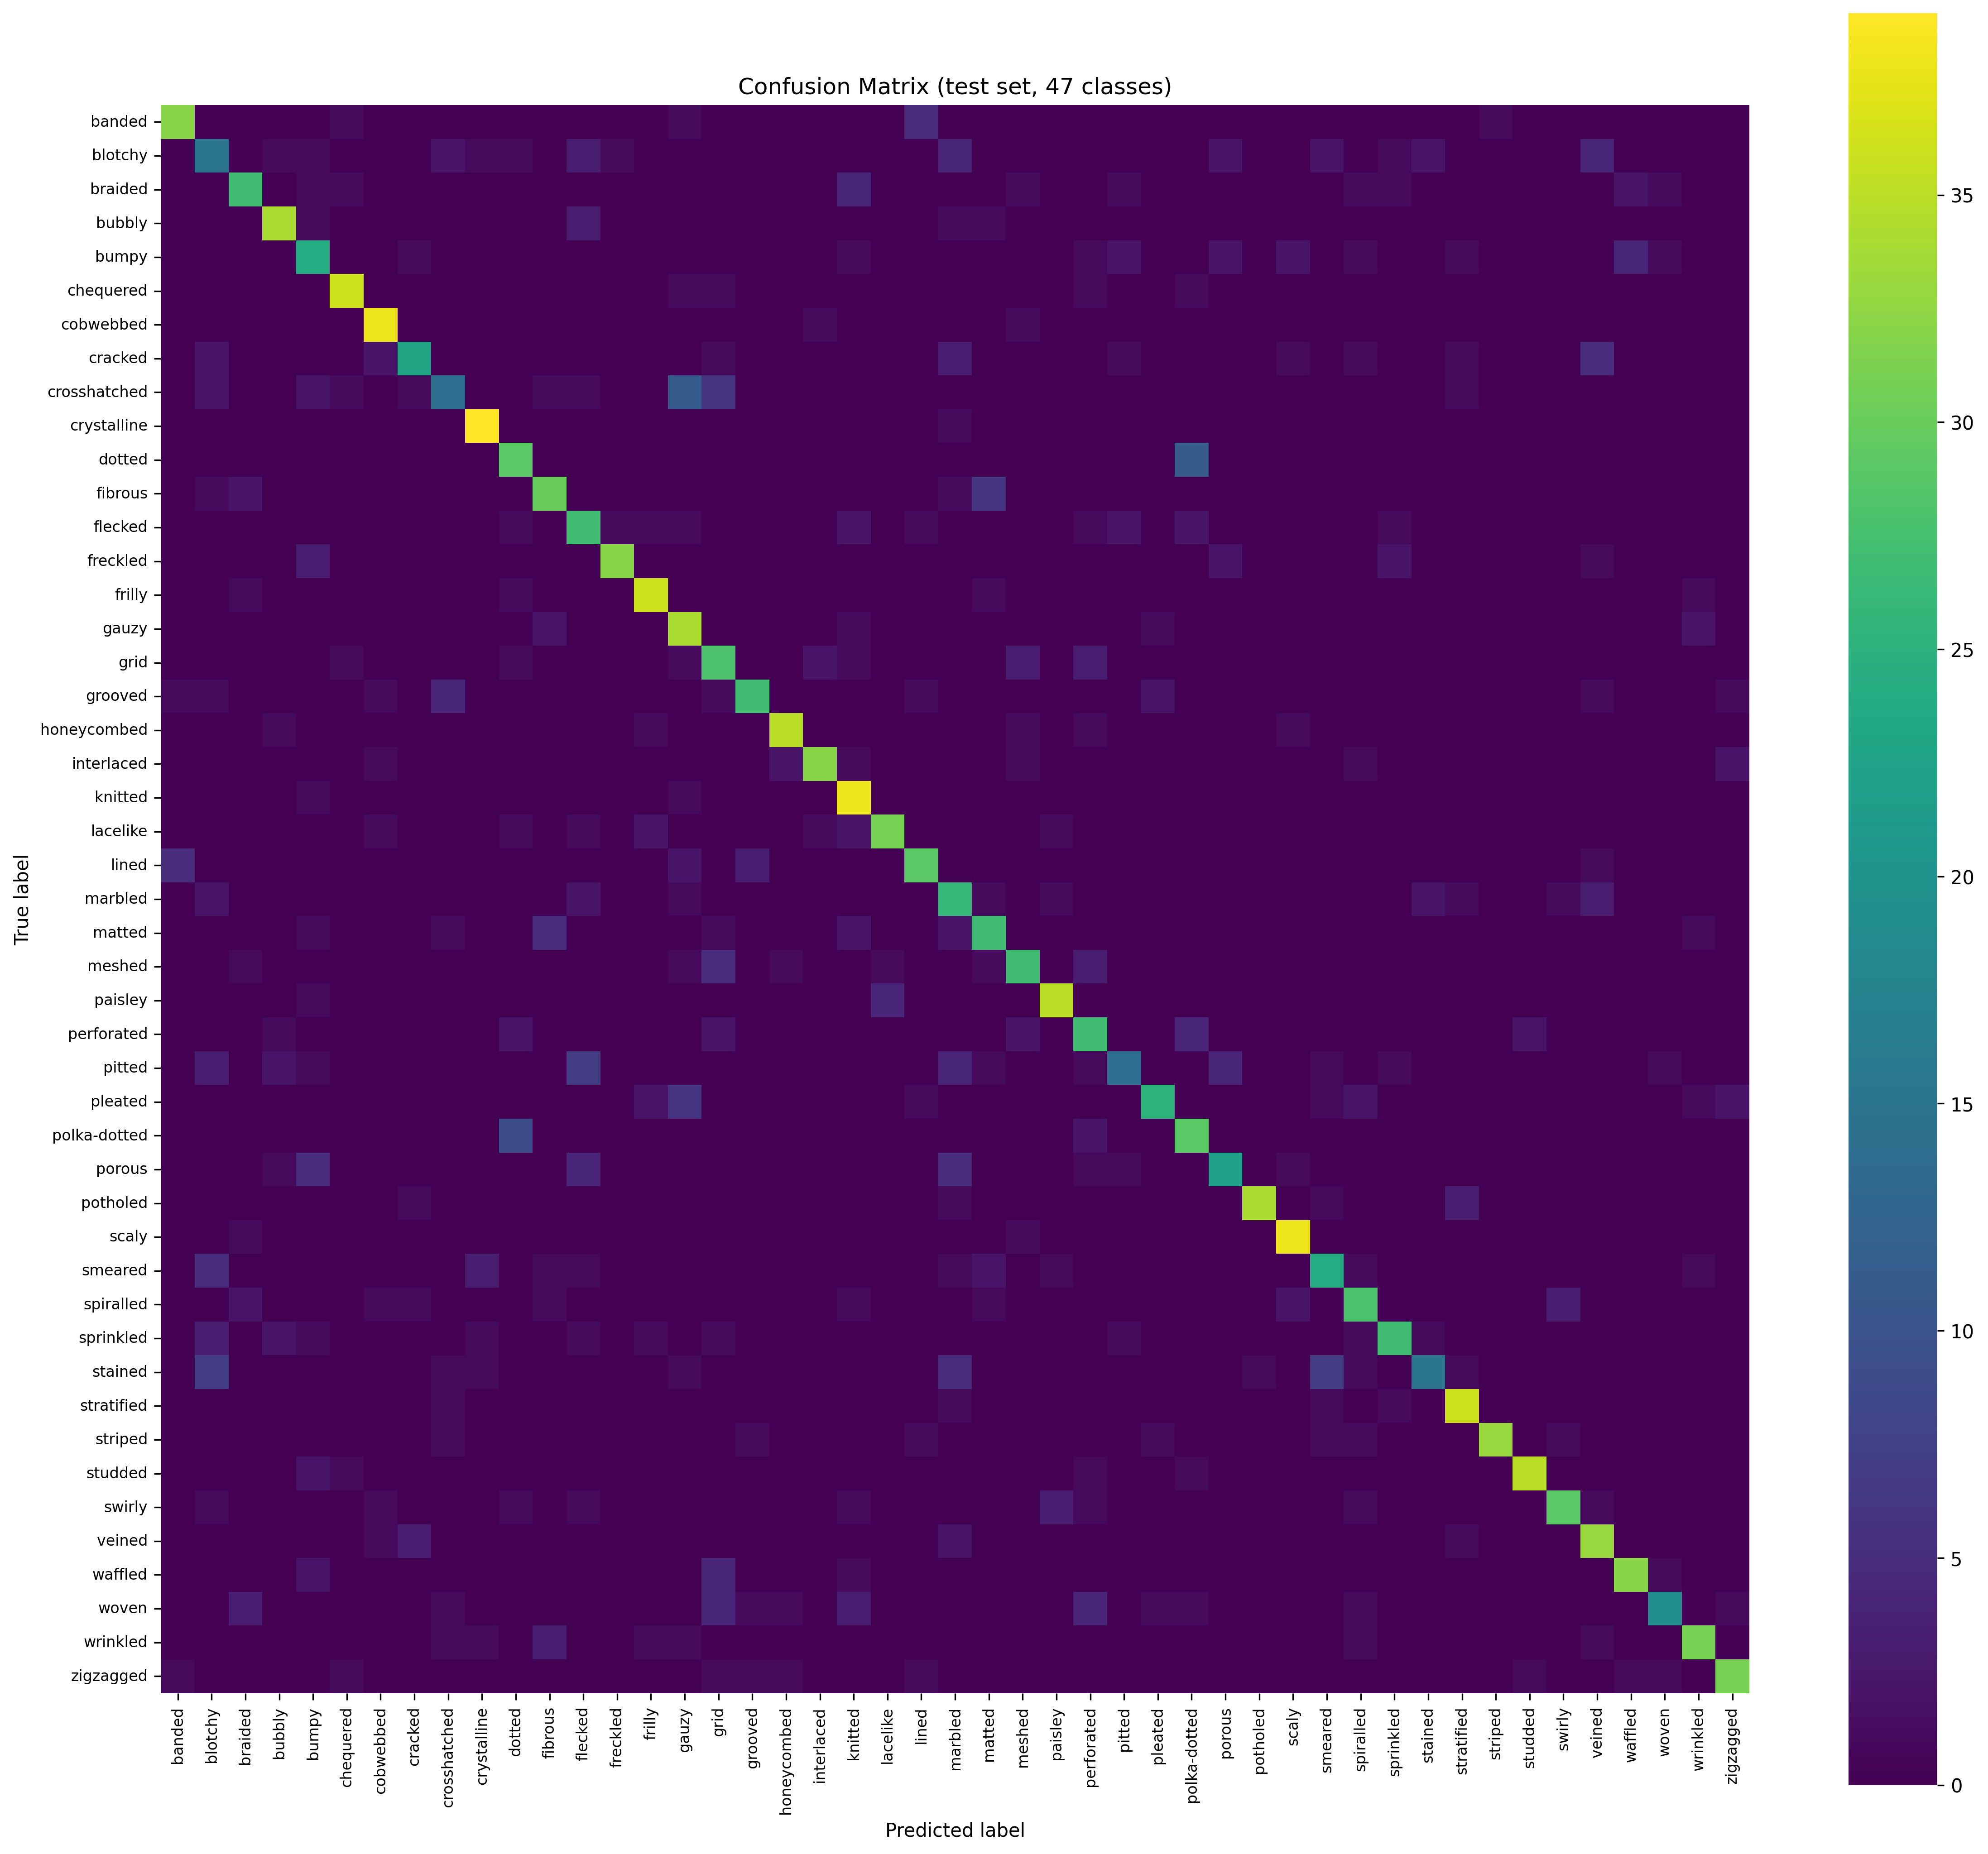
\includegraphics[height=4.2in]{output/confusion_matrix.png}
    \caption{Training/validation curves and test-set confusion matrix. The strong diagonal confirms good overall classification; most mistakes are scattered among visually related texture categories such as dotted/polka-dotted, grid/lined/crosshatched, and fibrous/matted/woven patterns.}
    \label{fig:results}
\end{figure}

\end{document}
